
\section{Introduction}
This document describes how to use the \LaTeX2e class file, named 
``{\tt scitrans.cls}'', for Transactions of the Institute of Systems, 
Control and Information Engineers (ISCIE). 

{\tt scitrans.cls} works together with the following nine files: 
\begin{itemize}
\item {\tt scitrans.cls}
\item {\tt sci209.sty, scij.sty, scie.sty, scims.sty}
\item {\tt JT1scimc.fd, JT1scigt.fd}
\item {\tt JY1scimc.fd, JY1scigt.fd}
\end{itemize}
Please make sure that all these files are placed in the same directory 
as the source file and should not be modified.


\section{Sections, etc.}
This is an example of \verb+\section{ }+.

\subsection{Subsections}
This is an example of \verb+\subsection{ }+.

\subsubsection{Sub-Subsections}
This is an example of \verb+\subsubsection{ }+.


\paragraph{Paragraphs}
This is an example of \verb+\paragraph{ }+.
Please insert a blank line before \verb+\paragraph{ }+.


\subparagraph{Subparagraphs}
This is an example of \verb+\subparagraph{ }+.
Please insert a blank line before \verb+\subparagraph{ }+.


\section{Theorems, etc.}
In the {\tt scitrans.cls} class file,
theorems and related structures such as definition, lemma, proposition,
corollary, example, assumption, remark and proof are handled. 
For example,

\begin{theorem}
\label{theorem:1}
This is an example of the theorem environment.
The usage of the lemma, definition, proposition, corollary,
example and assumption environments 
are the same as that of the theorem environment.
\end{theorem}

\begin{proof}
This is an example of the proof environment. 
At the end of each proof, asterisks ``**'' are automatically placed
as the Q.E.D.\ symbol,
whereas they will be replaced by the symbol ``$\Box$'' in the final manuscript.
\end{proof}

\begin{remark}
\label{remark:1}
This is an example of the remark environment. 
\end{remark}

If the author wishes to declare a new theorem-like environment, 
\verb+newtheoremenv+ and \verb+newparenenv+ can be used.
For example,

\begin{newtheoremenv}{Question}
This is an example of declaring a new environment by \verb+newtheoremenv+.
\end{newtheoremenv}
\begin{newparenenv}{Answer}
This is an example of declaring a new environment by \verb+newparenenv+.
\end{newparenenv}



\section{Equations}
Equations are created by the traditional {\tt equation} environment. 
In order to produce multiline equations,
the {\tt eqnarray} environment can be used.
For example, 

\begin{eqnarray}
        \dot{\mbf{x}}(t) & = & A \mbf{x}(t) + B \mbf{u}(t) 
                               + \sum_{k=1}^N \Gamma_k \mbf{d}k(t)
                \label{eq:1}\\
        \mbf{y}(t) & = & C \mbf{x}(t) + D \mbf{u}(t)
                \label{eq:2}\\
        \mbf{u}(t) & = & F \mbf{x}(t)
                \label{eq:3}
\end{eqnarray}

\begin{subequations}  \label{eq:4}  
  \begin{eqnarray}
    \lefteqn{ 
        \frac{1}{2\pi} \int_{-\infty}^\infty 
        {\rm Tr}\, \{ \mbf{G}\T(-j\omega) \mbf{G}(j\omega) \} \, d\omega 
     }    \hspace*{2\zw} \nonumber \\
    & = & 
    \frac{1}{2\pi} \int_{-\infty}^\infty 
    {\rm Tr}\, \{  B\T (-j\omega I -A\T)^{-1}C\T \nonumber \\
    &   & 
    \times C (j\omega I - A)^{-1}B \}\, d\omega 
               \label{eq:4a} \\
    & = & 
    \frac{1}{2\pi j}\int_{-j\infty}^{j\infty} 
    {\rm Tr}\, \left\{ 
    \left[ \begin{array}{c|c} 
       A & B \\ \hline 
       C & 0 \end{array} \right]^\sim  
    \left[ \begin{array}{c|c} 
       A & B \\ \hline 
       C & 0 \end{array} \right]
    \right\} \, ds  
              \label{eq:4b} 
\end{eqnarray}
\end{subequations}

In multiline equations,
please pay attention to the message ``\verb+Overfull \hbox+'', 
and the equations should be composed with the proper length.

With the \verb+subequations+ environment, sub-equation numbers such as 
\Req{eq:4a}, \Req{eq:4b} can be achieved.
In equations, bold fonts can be output by using \verb+\mbf+ command.
The superscript ${\rm T}$ which expresses the transpose of a matrix and $\hinf$ 
can be achieved by \verb+\T+ and \verb+\hinf+ respectively.

For in-line equations, please use $\displaystyle \sum_{k=1}^N$
instead of $\sum_{k=1}^N$.
Similarly, the rule is applicable to \verb+\lim+, \verb+\max+, \verb+\min+,
etc.
For super and subscripts,
please use $X_a^b$ (\verb+$X_a^b$+) instead of ${X_a}^b$ (\verb+${X_a}^b$+).


\section{Figures and Tables}
%----------------------------
\begin{figure}[b]
        \centering
	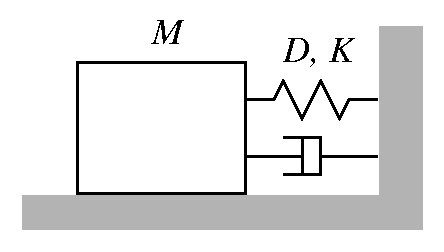
\includegraphics[width=5cm,clip]{tmp.eps}
        \caption{Mass-spring-damper system}
        \label{fig:1}
\end{figure}
%----------------------------
%
%----------------------------
\setlength{\unitlength}{10mm}
%

\begin{figure}[b]
        \centering
%
        \begin{picture}(4.5,1)(0,0)
                \thicklines
                \put(0,0.5){\vector(1,0){1.5}}
                \linethickness{1.2pt}
                \put(1.5,0){\framebox(1.5,1){$G(s)$}}
                \thicklines
                \put(3,0.5){\vector(1,0){1.5}}
        \end{picture}
%
        \caption{Plant}
        \label{fig:2}
\end{figure}
%----------------------------
%
%----------------------------
\begin{figure}[b]
        \centering
%
        \begin{picture}(5.5,2.5)(0,0)
                \thicklines
                \put(0,2){\vector(1,0){0.85}}
                \put(0.7,2.2){\makebox(0,0){$ \scriptstyle + $}}
                \put(1,2){\circle{0.3}}
                \thicklines
                \put(1.15,2){\vector(1,0){0.85}}
                \linethickness{1.2pt}
                \put(2,1.5){\framebox(1.5,1){$G(s)$}}
                \thicklines
                \put(3.5,2){\line(1,0){1}}
                \put(4.5,2){\circle*{0.08}}
                \put(4.5,2){\vector(1,0){1}}
                \put(4.5,2){\line(0,-1){1.5}}
                \put(4.5,0.5){\vector(-1,0){1}}
                \linethickness{1.2pt}
                \put(2,0){\framebox(1.5,1){$H(s)$}}
                \thicklines
                \put(2,0.5){\line(-1,0){1}}
                \put(1,0.5){\vector(0,1){1.35}}
                \put(0.8,1.7){\makebox(0,0){$ \scriptstyle - $}}
        \end{picture}
%
        \caption{Feedback control system}
        \label{fig:3}
\end{figure}

Graphics files (EPS files) can be inserted into a manuscript by 
\verb+\includegraphics+ command of the {\tt graphicx} package
(see \rfig{fig:1}). 
Here are some examples to insert graphics into a manuscript.
The {\tt picture} environment is also available
to draw figures (see \rfig{fig:2,fig:3}).

%
\begin{table}[h]
  \centering
  \caption{Example of table ({\tt slashbox.sty})}
  \label{table:1}
        \vspace{0.5\baselineskip}
  \begin{tabular}{!l!*{2}{c|}c!}\hlinethick
  \backslashbox{Room}{Date}
    &\makebox[3em]{5/31} &\makebox[3em]{6/1} &\makebox[3em]{6/2}\\ \hlinethick
    Room A	& --- & --- & --- \\ \hline
    Room C12	& --- & --- & --- \\ \hline
    Room F1201	& --- & --- & --- \\ \hlinethick
  \end{tabular}
\end{table}
%

Here is an example of a table. 
In the {\tt scitrans.cls},
the \verb+\tabular+ command has been extended for the ISCIE format.
The \verb+\tabular+ command provides the thin and thick lines.
The thin line can be achieved by the traditional way: ``\verb+|+''
for the vertical line and ``\verb+\hline+'' for the horizontal line.
The thick line can be achieved by ``\verb+!+'' and ``\verb+\hlinethick+''
for the vertical and horizontal thick lines respectively.

The {\tt arydshln.sty} is included in the {\tt scitrans.cls}
so that dashed lines are also available. 
Examples are shown in \rtab{table:2,table:3}.

%----------------------------
\begin{table}[hbt]
        \centering
        \caption{Commands for reference}
        \label{table:2}

        \vspace{0.5\baselineskip}

        \hdashlinewidth=8pt
        \hdashlinegap=4pt
        \begin{tabular}{!c|l!} \hlinethick
                Definition  & \verb+\rdefinition+ \\ \hdashline
                Theorem     & \verb+\rtheorem+ \\ \hdashline
                Lemma       & \verb+\rlemma+ \\ \hdashline
                Proposition & \verb+\rproposition+ \\ \hdashline
                Corollary   & \verb+\rcorollary+ \\ \hdashline
                Example     & \verb+\rexample+ \\ \hlinethick
        \end{tabular}
\end{table}
%----------------------------
%
%
%----------------------------
\begin{table}[hbt]
        \centering
        \caption{Commands for reference to equations, figures and tables}
        \label{table:3}

        \vspace{0.5\baselineskip}

        \hdashlinewidth=2pt
        \hdashlinegap=2pt
        \begin{tabular}{!l|l!} \hlinethick
                Equation                 & \verb+\req+ \\ \hdashline
                Equation in appendices   & \verb+\Req+ \\ \hdashline
                Equation with sub-number & \verb+\Req+ \\ \hdashline
                Figure                   & \verb+\rfig+ \\ \hdashline
                Table                    & \verb+\rtab+ \\ \hlinethick
        \end{tabular}
\end{table}
%----------------------------


\section{Citations}
Citations can be made with the \verb+\cite+ command\cite{foo1}. 
The \verb+\cite*+ command automatically places a word ``Ref.''
before the reference number as ``\cite*{foo1}''.

The multiple citation such as
\verb+\cite{foo1,foo2}+ and \verb+\cite{foo2,foo3,foo4}+ 
achieves \mbox{}\cite{foo1,foo2} and \mbox{}\cite{foo2,foo3,foo4} respectively.


\section{Cross-Referencing}
In order to reference the definition, theorem etc.,
please use the commands listed in \rtab{table:2},
for example: \verb+\rtheorem{theorem:1}+, \verb+\rremark{remarl:1}+.

\rtheorem{theorem:1} is an example of the \verb+\rtheorem+ command.

\rremark{remark:1} is an example of the \verb+\rremark+ command.

For referencing the equation,
figure and table, please use the commands listed in \rtab{table:3}.
These commands automatically add appropriate words before reference numbers.
For example, 
%the commands \verb+\req{eq:1}+, \verb+\rfig{fig:1}+ and \verb+\rtab{table:1}+
achieve 

\begin{itemize}
  \item \verb+\req{eq:1}+ $\quad\Longrightarrow\quad$ \req{eq:1}
  \item \verb+\rfig{fig:1}+ $\quad\Longrightarrow\quad$ \rfig{fig:1}
  \item \verb+\rtab{table:1}+ $\quad\Longrightarrow\quad$ \rtab{table:1}
\end{itemize}
The multiple referencing can be also achieved, for example,
\begin{itemize}
  \item \verb+\req{eq:1,eq:2,eq:3}+ $\quad\Longrightarrow\quad$
	\req{eq:1,eq:2,eq:3}
  \item \verb+\rfig{fig:1,fig:2}+ $\quad\Longrightarrow\quad$ \rfig{fig:1,fig:2}
  \item \verb+\rtab{table:1,table:2}+ $\quad\Longrightarrow\quad$
	\rtab{table:1,table:2}
\end{itemize}
In order to use the same format through the manuscript,
please do not use traditional 
\verb+\ref+ command.


\section{Others}
\subsection{Footnote}
The footnote is available with \verb+\footnote+ command%
\footnote{This is an example of the {\tt \textbackslash footnote} command.}.

\subsection{URL}
The {\tt scitrans.cls} provides the \verb+\url+ command to output a URL. 
For example, \url{http://www.iscie.or.jp/} can be achieved by 
\verb+\url{http://www.iscie.or.jp/}+. 
Also, {\tt \url{http://www.iscie.or.jp/}}  can be achieved by 
\verb+{\tt \url{http://www.iscie.or.jp/}}+. 


\acknowledgement
The \verb+\acknowledgement+ command can be used to state the acknowledgements. 


\begin{thebibliography}{9}
\bibitem{foo1}
        I.\ S.\ Cie: 
        The ISCIE style option; 
        {\it ISCIE Journal}, Vol.~0, No.~0, pp.~000--999 (1999)

\bibitem{foo2}
        R.\ E.\ Kalman: 
        A New Approach to Linear Filtering and Prediction Problems; 
        {\it Trans.\ of the ASME--J. of Basic Engineering}, Vol.~82 (Series D), 
        pp.~35--45 (1960)

\bibitem{foo3}
        A.\ Papoulis: 
        {\it Probability, Random Variables and Stochastic Processes}; 
        4th Edition, McGraw-Hill (2002)

\bibitem{foo4}
        Authors:
        Article title, {\it Book Title} (Editor(s), Ed(s).), Publisher,
        pp.~00--99 (1999)
\end{thebibliography}



%% Appendix
%
\appendix

This is an example of the \verb+\appendix+ command.
If there is only one section, please use \verb+\section*+ command. 
If there is more than one section, please use \verb+\section+ command.

\section{Equation in Appendix}
This is an example of \verb+\section+ command in the appendix. 
\begin{equation}
  u=Fx
\end{equation}

\section{Slash Line in Table}
In {\tt scitrans.cls}, {\tt slashbox.sty} is included so that slash 
lines are available in tables.
The followings are quoted from the manual of {\tt slashbox.sty} which is 
slightly modified for this document.

The usage is pretty straightforward, such as

\bigskip  %%Do not use this command in your manuscript.

\begin{tabular}{!l!*{3}{c!}}\hlinethick
\backslashbox{Room}{Date}
&\makebox[3em]{5/31}&\makebox[3em]{6/1}&\makebox[3em]{6/2}\\ \hlinethick
Room A&&&\\ \hline
Room C12&&&\\ \hline
Room F102&&&\\ \hlinethick 
\end{tabular}

\bigskip  %%Do not use this command in your manuscript.

\noindent
You may include a newline (\verb+\\+) in `Room' and/or `Date'.
Note that you will get spaces aside the slash line if there is a
wider column in the same column of a different line.
In such a case, you need to specify the width of the slashed column
by saying

\bigskip  %%Do not use this command in your manuscript.

\begin{tabular}{!l!*{2}{c!}} \hlinethick 
\backslashbox[40mm]{Room}{Date}
&\makebox[3em]{5/31}&\makebox[3em]{6/1}\\ \hlinethick 
Long Long Room Name&&\\ \hline
Room C12&&\\ \hline
Room F102&&\\ \hlinethick
\end{tabular}

\bigskip  %%Do not use this command in your manuscript.

The specified width is ignored if it is narrower than the natural
width of the column.

\verb+\(back)slashbox+ assumes by default that there is a blank space
of width \verb+\tabcolsep+ on both sides of the column.
Thus the slash line might exceed the boundary when you use \verb+@{}+ 
etc.

You can avoid it by specifying

\bigskip  %%Do not use this command in your manuscript.

\begin{tabular}{!@{\ $\bullet$\hspace*{3mm}}l!*{3}{c!}} \hlinethick 
\multicolumn{1}{!@{}l!}{\backslashbox[0pt][l]{Room}{Date}}
&\makebox[3em]{5/31}&\makebox[4em]{6/1}&\makebox[3em]{6/2}\\ \hlinethick
Room A&&&\\ \hline
Room C12&&&\\ \hline
Room F102&&&\\ \hlinethick 
\end{tabular}

\bigskip  %%Do not use this command in your manuscript.

\noindent
Here \verb+[l]+ tells the command that there is no extra space on the
left of this column.  You can use \verb+[r]+ and \verb+[lr]+ likewise.
You have to also specify the width of the column in this case, but it
can be 0pt.


\bigskip  %%Do not use this command in your manuscript.



\chosharyakureki

\authorbiography{Given-name, ,Family-name}{}{Member}{%
  Example of {\tt \textbackslash authorbiography}
  command. If you wish to include your photograph, please use this command.
  Please submit your photo after acceptance for publication.
  Please write down your biography here....
  Please write down your biography here....
  Please write down your biography here....
  Please write down your biography here....
  Please write down your biography here....
  Please write down your biography here....
  }

\authorbiography{Given-name, ,Family-name}{}{Non-Member}{%
  Example of {\tt \textbackslash authorbiography}
  command. If you wish to include your photograph, please use this command.
  Please submit your photo after acceptance for publication.
  Please write down your biography here....
  Please write down your biography here....
  Please write down your biography here....
  Please write down your biography here....
  Please write down your biography here....
  Please write down your biography here....
  }

\authorbiography*{Given-name, ,Family-name}{}{Member}{%
  Example of {\tt \textbackslash authorbiography$\ast$} command.
  If you do not wish to include your photograph, please use this command.
  Please write down your biography here....
  Please write down your biography here....
  Please write down your biography here....
  Please write down your biography here....
  }
